\chapter{Literature Review and Background}

In this thesis, I have presented two way approach to improving the existing systems of recommender systems.
First, I have utilized the ratings present in the dataset corresponding to each purchase made by some user x of some product i to predict and recommend the items for some other user y using item-item based collaborative filtering. Secondly, LDA was used to extract topic modelling based words and features from the reviews left by the users on the products.

\section{\textit{k} Nearest Neighbour}
$k$ nearest neighbor or kNN classification determines the decision boundary locally. For 1NN we assign each document to the class of its closest neighbour. For kNN we assign each document to the majority class of its k closest neighbors where k is a parameter. The rationale of kNN classification is that, based on the contiguity hypothesis, we expect a test document $d$ to have the same label as the training documents located in the local region
surrounding $d$.

For general, k ∈ N in kNN, consider the region in the space for which the set of k nearest neighbors is the same. This again is a convex polygon and the space is partitioned into convex polygons, within each of which the set of k nearest neighbours is invariant.
The parameter k in kNN is often chosen based on experience or knowledge about the classification problem at hand.  It is desirable for k to be odd to make ties less likely. k = 3 and k = 5 are common choices, but much larger values between 50 and 100 are also used.  An alternative way of setting the parameter is to select the k that gives best results on a held-out portion of the training set.
\begin{figure}[H]
    {\centering {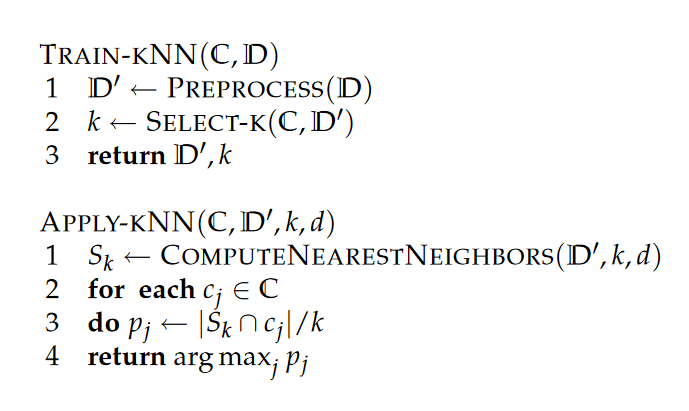
\includegraphics[width = 0.7 \textwidth]{img/kNNtrain}}\par}
    \caption{kNN  training(with preprocessing) and testing. $p_{j}$ is an estimate for $P(c_{j}|S_{k}) = P(c_{j}|d)$. $c_{j}$ denotes the set of all documents in the class $c_{j}$.}
\end{figure}

\section{Matrix Factorization | Singular Valued Decomposition | LSA }
The square decompositions are simpler and can be treated with sufficient mathematical rigor to help understand how such decompositions work. Square symmetric matrices is the basis of the singular valued decomposition.

In LSI, we use SVD to construct a low-rank approximation matrix C, to the term-document matrix, for a value of k that is far smaller than original rank of C. 

\subsection{Term-document matrices and Singular value Decomposition}
However, the matrix we are interested in is the M × N term-document matrix C where (barring a rare coincidence) M 6 = N ;furthermore, C is very unlikely to be symmetric. To this end, we first describe an extension of the symmetric diagonal decomposition known as the singular value decomposition.

Given an M × N matrix C and  a positive  integer k ,  we  wish  to  find  an M × N matrix C k of rank at most k , so as to minimize the Frobenius norm of F RO BENI US NO RM the matrix difference X = C − C k , defined to be

\[
    \| X_{F} \| = \sqrt{\sum_{i=1}^{M} \sum_{j=1}^{N} X_{ij}^2}
\]

Thus, the Frobenius norm of X measures the discrepancy between C k and C ; our goal is to find a matrix C k that minimizes this discrepancy, while con- straining C k to have rank at most k .   If r is the  rank of C ,  clearly C r = C and the Frobenius norm of the discrepancy is zero in this case . When k is far smaller than r , we refer to C k as a low-rank approximation. The singular value decomposition can be used to solve the low -rank ma- trix approximation problem.   We then derive from it an applic ation to ap- proximating term-document matrices.

The singular value decomposition can be used to solve the low -rank ma- trix approximation problem.   We then derive from it an applic ation to ap- proximating term-document matrices.   We invoke the followi ng three-step procedure to this end:

\begin{figure}[H]
    {\centering {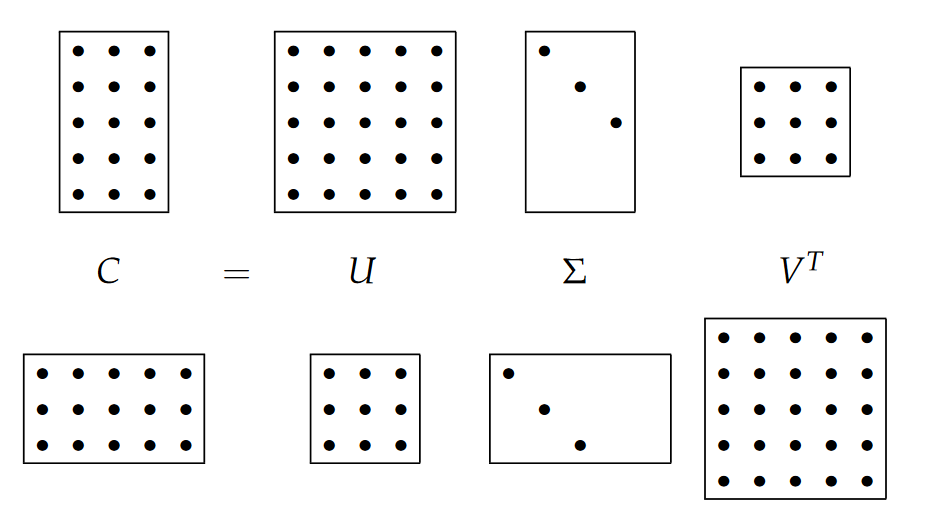
\includegraphics[width = 0.9 \textwidth]{img/SVD}}\par}
    \caption{Svd}
\end{figure}


1. Given C , construct its SVD in the form shown in ( 18.9 ); thus, C = U Σ V T . 2. Derive from Σ the matrix Σ k formed by replacing by zeros the r − k small- est singular values on the diagonal of Σ . 3. Compute and output C k = U Σ k V T as the rank- k approximation to C . The rank of C k is at most k :  this follows from the fact that Σ k has at most k non-zero values.  Next, we recall the intuition of Example 18.1 :  the effect of small eigenvalues on matrix products is small.  Thus, it se ems plausible that replacing these small eigenvalues by zero will not subs tantially alter the product, leaving it “close” to C .  The following theorem due to Eckart and Young tells us that, in fact, this procedure yields the matri x of rank k with the lowest possible Frobenius error.

\section{Latent Factor Topic Modelling | Text Clustering}

% \begin{figure}[h]
%    {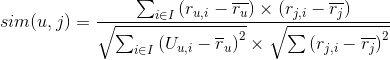
\includegraphics[scale=1]{img/PearsonEqn.png}}
% \end{figure}
Topic Modelling has been a way to comprehend text for the machine learning community. This can be of supervised or unsupervised nature. For the task of this thesis, we have employed the unsupervised version of the topic modelling. A number of simple unsupervised methods can be used for feature selection in text clustering. Some examples of such methods are discussed below.

\subsection{Document Frequency-based Selection}
The simplest possible method for feature selection in document clustering is that of the use of document frequency to filter out irrelevant features. While the use of inverse document frequencies reduces the importance of such words, this may not alone be sufficient to reduce the noise effects of very frequent words. In other words, words which are too frequent in the corpus can be removed because they are typically common words such as "a", "an", "the", or "of" which are not discriminative from a clustering perspective. Such words are also referred to as stop words. A variety of methods are commonly available in the literature for stop-word removal. Typically commonly available stop word lists of about 300 to 400 words are used for the retrieval process. In addition, words which occur extremely infrequently can also be removed from the collection. This is because such words do not add anything to the similarity computations which are used in most clustering methods. In some cases, such words may be misspellings or typographical errors in documents. Noisy text collections which are derived from the web, blogs or social networks are more likely to contain such terms. We note that some lines of research define document frequency based selection purely on the basis of very infrequent terms, because these terms contribute the least to the similarity calculations. However, it should be emphasized that very frequent words should also be removed, especially if they are not discriminative between clusters. Note that the TF-IDF weighting method can also naturally filter out very common words in a “soft” way. Clearly, the standard set of stop words provide a valid set of words to prune. There are other ways of quantifying the important words directly to the clustering process, which is essential to more aggressive pruning.

\subsection{Term Strength}
A much more aggressive technique for stop-word removal has been proposed in \cite{Wilbur1992}. The core idea of this approach
is to extend techniques which are used in supervised learning to the unsupervised case. The term strength is essentially used to measure how informative a word is for identifying two related documents. For example, for two related documents x and y, the term strength $s(t)$ of term $t$ is defined in terms of the following probability:
\[
    s(t) = P(t \in y | t \in x)
    \label{eq:probTermStrength} \tag{233}
\]

Clearly, the main issue is how one might define the document x and y as related. One One possibility is to use manual (or user) feedback to define when a pair of documents are related. This is essentially equivalent to utilizing supervision in the feature selection process, and may be practical in situations in which predefined categories of documents are available. On the other hand, it is not practical to manually create related pairs in large collections in a comprehensive way. It is therefore desirable to use an automated and purely unsupervised way to define the concept of when a pair of documents is related. It has been shown in [94] that it is possible to use automated similarity functions such as the cosine function [81] to define the relatedness of document pairs. A pair of documents are defined to be related if their cosine similarity is above a user-defined threshold. In such cases, the term strength s(t) can be defined by randomly sampling a number of pairs of such related documents as follows:

\[
s(t) = \frac{\text{Number of pairs in which $t$ occurs in both}} {\text{Number of pairs in which $t$ occurs in the first of the pair}}
\label{eq:samplingpairs} \tag{234}
\]
Here, the first document of the pair may simply be picked randomly. In order to prune features, the term strength may be compared to the expected strength of a term which is randomly distributed in the training documents with the same frequency. If the term strength of t is not at least two standard deviations greater than that of the random word, then it is removed from the collection.
One advantage of this approach is that it requires no initial supervision or training data for the feature selection, which is a key requirement in the unsupervised scenario. Of course, the approach can also be used for feature selection in either supervised clustering \cite{Bobadilla2013} or categorization\cite{Salakhutdinov2007}, when such training data is indeed available. One observation about this approach to feature selection is that it is particularly suited to similarity-based clustering because the discriminative nature of the underlying features is defined on the basis of similarities in the documents themselves.

\subsection{Term Contribution}
The concept of term contribution \cite{Liu2003} is based on the fact that the results of text clustering are highly dependent on document similarity. Therefore, the contribution of a term can be viewed as its contribution to document similarity. For example, in the case of dot-product based similarity, the similarity between two documents is defined as the dot product of their normalized frequencies. Therefore, the contribution of a term of the similarity of two documents is the product of their normalized frequencies in the two documents. This needs to be summed over all pairs of documents in order to determine the term contribution. As in the previous case, this method requires $O(n^2)$ time for each term, and therefore sampling methods may be required to speed up the contribution. A major criticism of this method is that it tends to favor highly frequent words without regard to the specific discriminative power within a clustering process. In most of these methods, the optimization of term selection is based on some pre-assumed similarity function (e.g., cosine). While this strategy makes these methods unsupervised, there is a concern that the term selection might be biased due to the potential bias of the assumed similarity function. That is, if a different similarity function is assumed, we may end up having different results for term selection. Thus the choice of an appropriate similarity function may be important for these methods.


\subsection{Latent Dirichlet Allocation}

PLSI provides a good basis for text analysis, but it has two prob- lems. First, it contains a large number of parameters that grows linearly with the number of documents so that it tends to overfit the training data. Second, there is no natural way to compute the probability of a document that was not in the training data. LDA includes a pro- cess for generating the topics in each document, thus greatly reducing the number of parameters to be learned and providing a clearly-defined probability for arbitrary documents. Because LDA has a rich generative model, it is also readily adapted to specific application requirements, which we describe in Section 5.
3.2.1 Model. Like PLSI, LDA is based on a hypothetical generative process for a corpus. A diagram of the graphical model showing how the different random variables are related is shown in Fig. 5.1. In the diagram, each random variable is represented by a circle (continuous) or square (discrete). A variable that is observed (its outcome is known) is shaded. An arrow is drawn from one random variable to another if the the outcome of the second variable depends on the value of the first variable. A rectangular plate is drawn around a set of variables to show that the set is repeated multiple times, as for example for each document or each token.

Choose the term probabilities for each topic. The distribution of terms for each topic i is represented as a multinomial
distribution Φ i , which is drawn from a symmetric Dirichlet distri-
bution with parameter β.

\textbf{there is formula here.. refer text mining book}

Choose the topics of the document. The topic distribu- tion for document d is represented as a multinomial distribution θ d , which is drawn from a Dirichlet distribution with parameters α. The Dirichlet distribution captures the document-independent popularity and the within-document burstiness of each topic.

\textbf{refer LDA in text mining book}

Choose the topic of each token. The topic z dn for each token index n is chosen from the document topic distribution.

\textbf{same here...text mining data}

Choose each token. Each token w at each index is chosen from the multinomial distribution associated with the selected topic.



\subsubsection{Mechanism} LDA provides the mechanism for finding patterns of term co-occurrence and using those patterns to identify coherent topics. Suppose that we have used LDA to learn a topic i and that for term v, p(w = v|z = i) is high. As a result of the LDA generative process, any document d that contains term v has an elevated probability for topic i, that is, p(z dn ? = i|w dn = v) > p(z dn ? = i). This in turn means that all terms that co-occur with term v are more likely to have been gen- erated by topic i, especially as the number of co-occurrences increases. Thus, LDA results in topics in which the terms that are most probable frequently co-occur with each other in documents. Moreover, LDA also helps with polysemy. Consider a term v with two distinct meanings in topics i and i ? . Considering only this term, the model places equal probability on topics i and i ? . However, if the other words in the context place a 90\% probability on i and only a 9\% probability on i ? , then LDA will be able to use the context to disambiguate the topic: it is topic i with 90\% probability.

Wallach et al. [60] show that the symmetry or asymmetry of the Dirichlet priors strongly influences the mechanism. For the topic-specific term distributions, a symmetric Dirichlet prior provides smoothing so that unseen terms will have non-zero probability. However, an asym- metric prior would equally affect all topics, making them less distinctive. In contrast, they showed that an asymmetric prior for the document- specific topic distributions made LDA more robust to stop words and less sensitive to the selection of the number of topics. The stop words were mainly relegated to a small number of highly probable topics that influence most documents uniformly. The asymmetric prior also results in more stable topics, which means that additional topics will make small improvements in the model instead of radically altering the topic structure. This is similar to the situation of LSI, where performance is optimal when Σ scales the contribution of each dimension according to its eigenvalue. In the same way, LDA will perform best if α is non- uniform and corresponds to some natural values characteristic of the dataset.
One disadvantage of LDA is that it tends to learn broad topics. Con- sider the case where a concept has a number of aspects to it. Each of the aspects co-occurs frequently with the main concept, and so LDA will favor a topic that includes the concept and all of its aspects. It will further favor adding other concepts to the same topic if they share the same aspects. As this process continues, the topics become more diffuse. When sharper topics are desired, a hierarchical topic model may be more appropriate.

\subsubsection{Likelihood} Training an LDA model involves finding the optimal set of parameters, under which the probability of generating the training documents is maximized. The probability of the training documents under a given sLDA model is called the empirical likelihood L. It can also be used to identify the optimal model configuration using Bayesian model selection.

\textbf{there is some equation}

Unfortunately, the direct optimization of the likelihood is problematic because the topic assignments z dn are not directly observed. Even inference for a single document is intractable. We describe two different approximations for LDA. Collapsed Gibbs sampling samples a value for each z dn in turn, conditioned on the topic assignments for the other to- kens. Variational Bayes approximates the model with a series of simpler models that bound the likelihood but neglect the troublesome dependencies.



